% !TeX root = ../main.tex
In questo capitolo viene descritto un caso d'uso aziendale di sviluppo di applicazione mobile adottando i metodi, gli automatismi e gli strumenti descritti nel capitolo \ref{ch:ch4}. L'obiettivo è quello di dimostrare l'efficacia del modello progettato tramite lo sviluppo di una applicazione mobile per la gestione e la visualizzazione dei contenuti digitali pubblicati da Maggioli SpA in formato ebook e rilasciata per le piattaforme Android e iOS.

\section{Analisi dei Requisiti}
\subsection{Requisiti Funzionali}
\begin{itemize}
    \item \textbf{R1} - Visualizzare documenti.
    \begin{itemize}
        \item \textbf{R1.1} - In modo fluido, mostrando il contenuto adattato al dispositivo in cui viene mostrato.
        \item \textbf{R1.2} - In modo statico, mostrando il contenuto con uno specifico layout indipendente dal dispositivo in cui viene mostrato.
    \end{itemize}
    \item \textbf{R2} - Modificare documenti in modo fluido (lato utente).
    \begin{itemize}
        \item \textbf{R2.1} - Aggiungere commenti, sottolineature, evidenziazioni, al contenuto fluido.
        \item \textbf{R2.2} - Memorizzare commenti, sottolineature, evidenziazioni apportate al contenuto fluido.
    \end{itemize}
    \item \textbf{R3} - Gestione utente.
    \begin{itemize}
        \item \textbf{R3.1} - Login (autenticazione) utente.
        \item \textbf{R3.2} - Visualizzare documenti a cui l'utente è abbonato.
    \end{itemize}
    \item \textbf{R4} - Ricerca documenti
    \begin{itemize}
        \item \textbf{R4.1} - Ricerca documenti senza autenticazione. Qualsiasi utente può effettuare una ricerca dei documenti disponibili, senza ottenere il contenuto.
        \item \textbf{R4.2} - Ricerca avanzata in base a diversi campi.
    \end{itemize}
    \item \textbf{R5} - Convertire documenti da modo statico a modo fluido.
    \item \textbf{R6} - Modificare documenti in modo fluido (lato azienda).
    \begin{itemize}
        \item \textbf{R6.1} - Aggiungere elementi/contenuti al documento in modo fluido (hyperlink, quiz, video, immagini, ...).
        \item \textbf{R6.2} - Memorizzare gli elementi/contenuti aggiunti al documento in modo fluido (hyperlink, quiz, video, immagini, ...).
    \end{itemize}
\end{itemize}

\subsection{Requisiti Non Funzionali/Tecnologici}
\begin{itemize}
    \item \textbf{T1} - Applicazione nativa Android e iOS, sfruttando Kotlin Multiplatform Mobile (KMM).
    \item \textbf{T2} - Continuous Integration e Continuous Delivery
    \begin{itemize}
        \item \textbf{T2.1} - Analisi statica del codice (SAST\footnote{Static Application Security Testing}).
        \item \textbf{T2.2} - Unit testing, code coverage e E2E\footnote{End-to-End} testing.
        \item \textbf{T2.3} - Rilascio automatico nei relativi store delle piattaforme scelte (Google Play per Android e App Store per iOS).
    \end{itemize}
    \item \textbf{T3} - Monitoraggio applicazione (Analytics).
\end{itemize}

\begin{figure}[H]
\centering
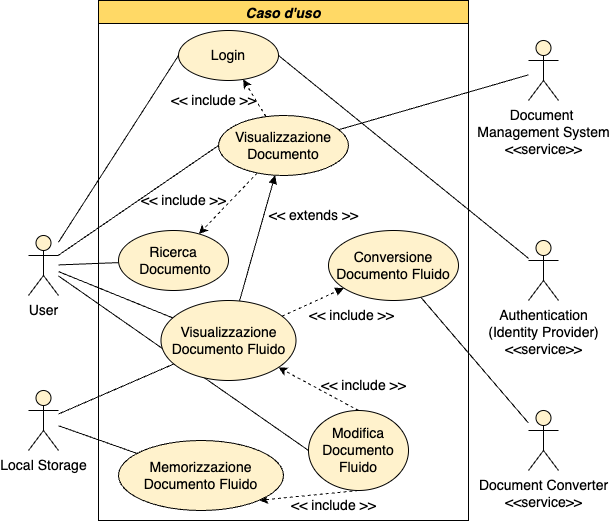
\includegraphics[width=0.8\textwidth]{img/tesi-1-Use-case.drawio.png}
\caption{Diagramma dei casi d'uso: funzioni/servizi offerti dal sistema Ebook App PoC}
\end{figure}

% indicare tramite le personas e le user story quali sono gli scenari d'utilizzo voluti dal committente (mauro e flower)
% io, come alala, vorrei, lalala

\begin{figure}[H]
\centering
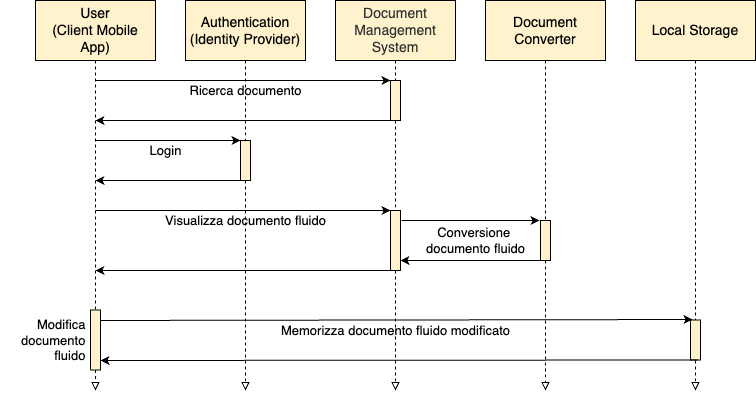
\includegraphics[width=1\textwidth]{img/tesi-2-Use-case2.drawio.png}
\caption{Diagramma di sequenza: scenario di modifica di un nuovo documento "fluido"}
\end{figure}


\section{Analisi Formati Digitali Fluidi}
I documenti attualmente sono reperibili in formato PDF e/o HTML. Il formato PDF è quello con cui i documenti vengono effettivamente archiviati: per ottenere un documento in formato HTML è necessario utilizzare un servizio interno, chiamato \textit{pdf2html}, il quale effettua la conversione. Entrambi i formati rispettano i requisiti per i documenti definiti "statici" ma non per quelli definiti "fluidi":
\begin{itemize}
    \item \textbf{PDF} (Portable Document Format) - Formato di file sviluppato da Adobe per rappresentare documenti di testo e immagini in modo indipendente dall'hardware e dal software utilizzati per generarli o per visualizzarli. Viene dunque generato e visualizzato con uno specifico layout.
    \item \textbf{HTML} (HyperText Markup Language) - Linguaggio di formattazione che descrive le modalità di impaginazione o visualizzazione grafica (layout) del contenuto, testuale e non, di una pagina web attraverso tag di formattazione. Viene generato tramite conversione del documento PDF riportando fedelmente il layout iniziale.
\end{itemize}
Per soddisfare i requisiti \textit{R1.1}, \textit{R2.1}, \textit{R5} e \textit{R6.1} il formato "fluido" deve:
\begin{itemize}
    \item rappresentare solamente il contenuto dei documenti "statici", rimuovendo tutte le formattazioni di layout,
    \item essere modificabile,
    \item poter essere ricavato convertendo un documento attualmente in formato "statico" (ovvero deve esistere un algoritmo/software per poter effettuare la conversione).
\end{itemize}
I formati attualmente disponibili che soddisfano i requisiti sopra indicati rappresentano implementazioni dello standard Open eBook (OeB), elaborato dall'Open E-book Forum. Tra questi i formati più diffusi sono:
\begin{itemize}
    \item \textbf{MOBI} (Mobipocket) - Standard proprietario (\textit{Amazon}) per la pubblicazione di libri digitali (eBook).\\
    Principali caratteristiche:
    \begin{itemize}
        \item basato sulla Open eBook standard utilizzando XHTML,
        \item annotazioni (highlights, segnalibri, correzioni, note e disegni) possono essere applicati, organizzati, e richiamati,
        \item può includere anche JavaScript e cornici.
    \end{itemize}
    \item \textbf{EPUB} (Electronic Publication) - Standard aperto specifico per la pubblicazione di libri digitali (eBook).\\
    Principali caratteristiche:
    \begin{itemize}
        \item basato sulla Open eBook standard utilizzando XML,
        \item a partire da settembre 2007 è lo standard ufficiale dell'International Digital Publishing Forum (IDPF)\footnote{\url{https://web.archive.org/web/20080827131750/http://www.idpf.org/2007/ops/OPS_2.0_final_spec.html}},
        \item CSS per il layout e la formattazione,
        \item testo "re-flowable" con grafica raster e vettoriale,
        \item disponibilità di diversi software, sia proprietari che open source, per la manipolazione del file (\textit{Adobe InDesign}, \textit{Sigil}, \textit{Calibre}, ...),
        \item disponibilità di tante librerie in diversi linguaggi per la manipolazione del file.
    \end{itemize}
\end{itemize}
Le caratteristiche determinanti che hanno portato alla scelta del formato EPUB sono state (\textit{i}) lo standard aperto e (\textit{ii}) la disponibilità, sia di software che di librerie, per la manipolazione del file. 

\section{Progettazione}
In questa sezione viene descritta la fase di progettazione del sistema, le cui attività principali consistono nella ($i$) modellazione del dominio e ($ii$) nella progettazione dell'interfaccia grafica tramite mockup.

\subsection{Modellazione Dominio}

L'obiettivo principale della applicazione è quello di permettere all'utente di "sfogliare" i contenuti digitali offerti da Maggioli sul proprio dispositivo. In questo caso si identificano quindi tre contesti:

\begin{itemize}
    \item \textit{Reader} (Core) - Contesto principale del progetto. Racchiude tutti gli aspetti con maggiore valore per l'utente riguardanti la lettura e personalizzazione dei contenuti digitali. 
    \item \textit{Sisred} - Rappresenta il contesto della sorgente dei contenuti digitali Maggioli (Sistema Redazionale\cite{amslaurea23043}). In questo contesto non esistono i concetti di \textit{favorite}, \textit{highlight}, \textit{bookmark} e \textit{progression} mentre è condiviso il concetto di libro e utente.
    \item \textit{User} - Contesto che definisce tutti gli aspetti a riguardo degli utenti. In questo contesto esiste il solo concetto di utente, il quale è condiviso con gli altri contesti.
\end{itemize}

\begin{figure}[H]
\centering
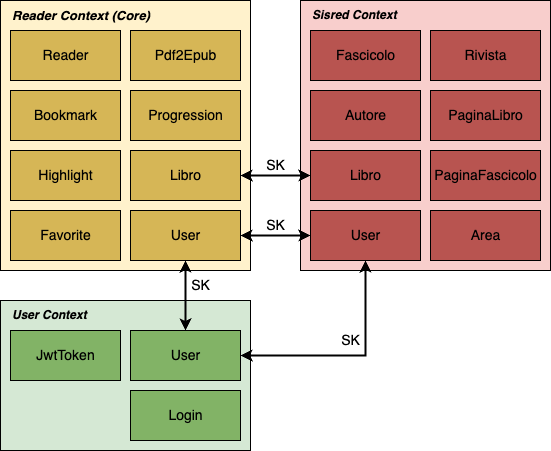
\includegraphics[width=0.7\textwidth]{img/tesi-20-app-domain.drawio.png}
\caption{Context Map: panoramica globale dei contesti del progetto e delle relazioni che intercorrono tra di essi}
\end{figure}

Tra i contesti definiti esistono delle relazioni di tipo \textit{Shared Kernel}\cite{evans_domain-driven_2004} (SK) con l'obiettivo di evitare duplicazioni e semplificare l'integrazione. Relazioni di questo tipo consistono nella condivisione di un sottoinsieme del dominio modellato, che corrisponde tipicamente al dominio core. Un esempio di relazione SK è l'utilizzo di codice o schemi DB condivisi\footnote{\url{https://github.com/ddd-crew/context-mapping}}.\\

Per la modellazione del dominio si fa uso dei seguenti concetti\cite{evans_domain-driven_2004}:
\begin{itemize}
    \item \textit{Entity} - Oggetto definito dalla sua identità e non dai suoi attributi. Ogni libro è univoco, identificato da uno specifico codice, chiamato ISBN\footnote{International Standard Book Number}.
    \item \textit{Value Object} - Al contrario delle entità, questi oggetti sono definiti dai loro attributi e non hanno una identità concettuale ma servono a descrivere alcune caratteristiche di un oggetto. Un esempio è il segnalibro: ciò che è rilevante è la pagina del libro che esso referenzia e non la sua identità.
    \item \textit{Aggregate} - Insieme di oggetti legati da una entità padre chiamata \textit{Root} (radice di aggregazione). L'aggregato composto da \textit{Bookmark}, \textit{Highlight}, \textit{Progression}, \textit{Favorite} ha come radice l'entità \textit{Libro}.
    \item \textit{Service} - Operazione che non appartiene logicamente a nessun oggetto. In questo caso la conversione di formato non appartiene alla sola entità libro ma appartiene invece a qualsiasi documento che è possibile convertire.
    \item \textit{Repository} - Oggetto per il recupero di altri oggetti di dominio e per la gestione del loro ciclo di vita. Le entità \textit{User} e \textit{Libro} sono esempi di oggetti di dominio che necessitano di un repository. Permette di disaccoppiare applicazione e domain design dalle specifiche tecnologie/strategie di persistenza come multipli database e datasource (locali e/o remoti).
\end{itemize}

\begin{figure}[H]
\centering
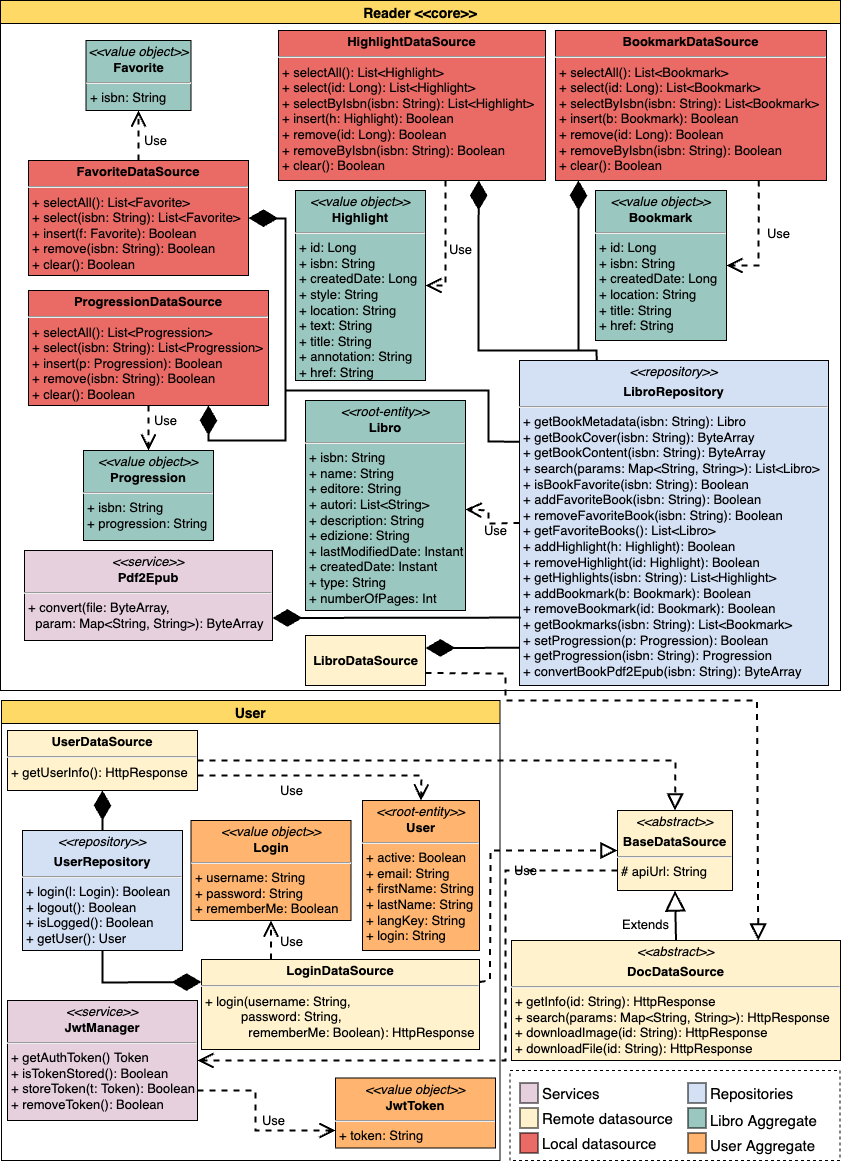
\includegraphics[width=0.9\textwidth]{img/tesi-25-ddd.drawio.png}
\caption{UML - Diagramma delle classi: Reader Core Domain e User Subdomain}
\label{fig:5.4}
\end{figure}

\subsection{Progettazione UI}

L'interfaccia grafica della applicazione è stata progettata tramite l'utilizzo di mockup digitali realizzati con il tool grafico open source Drawio\footnote{\url{https://github.com/jgraph/drawio}}. 

\begin{figure}[H]
\centering
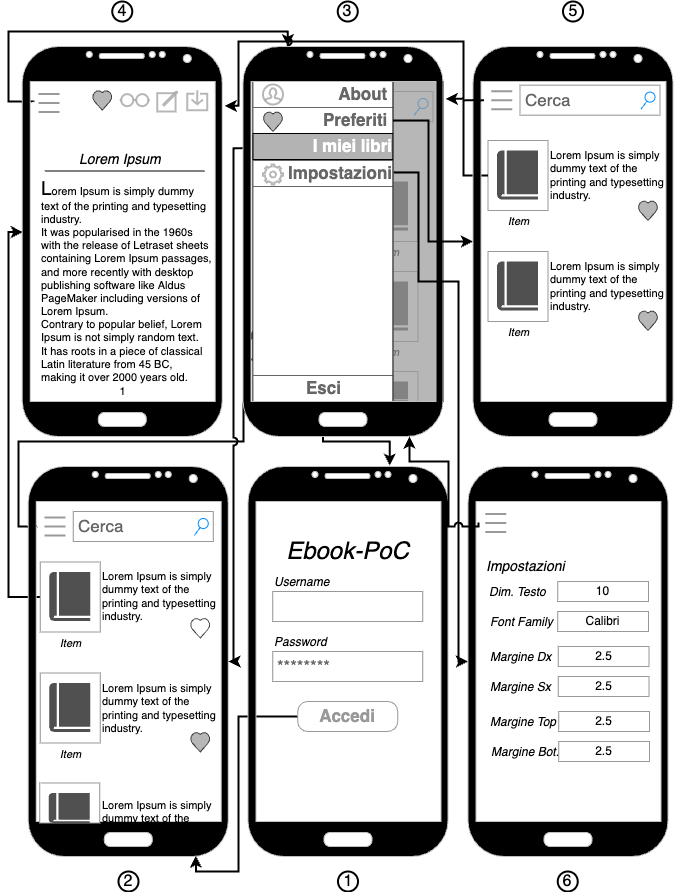
\includegraphics[width=0.8\textwidth]{img/tesi-14-mockup1.drawio.png}
\caption{Alcuni dei mockup realizzati per la progettazione e la validazione della UI (v1)}
\end{figure}

Considerando l'utilizzo tipico di una applicazione della stessa tipologia di quella che deve essere realizzata, sono stati utilizzati alcuni standard de-facto come ad esempio il menu laterale a scomparsa (mockup 4), icona "hamburger" per l'apertura del menu (mockup 3), elenco di elementi con scroll infinito verticale (schermata 5-6), barra di ricerca nella parte alta con icona "lente di ingrandimento" (schermata 2-5-6), ... .

\begin{figure}[H]
\centering
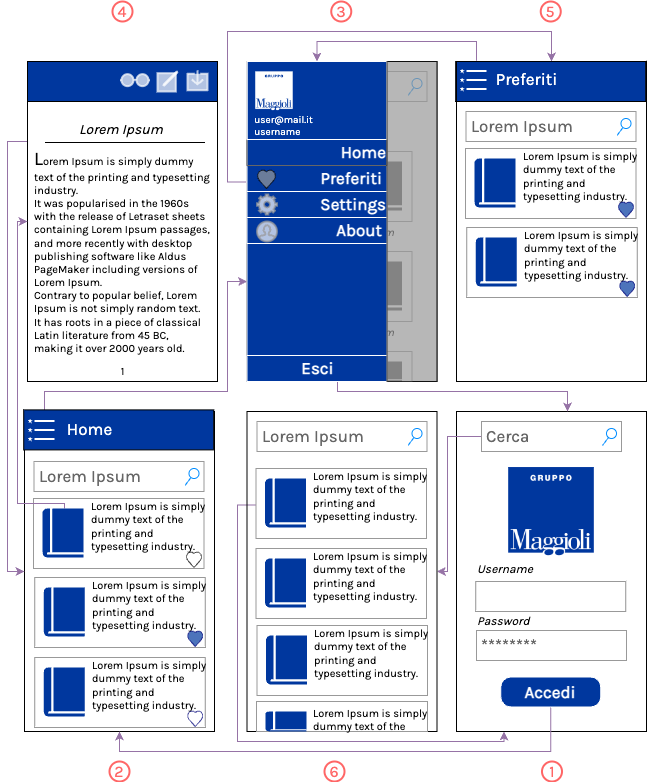
\includegraphics[width=0.8\textwidth]{img/tesi-23-mockupv2.drawio.png}
\caption{Modifiche apportate ai mockup per ottenere la validazione della UI (v2)}
\end{figure}

Sono state necessarie due iterazioni di validazione dei mockup da parte degli interessati per definire l'interfaccia utente desiderata con alcuni vincoli caratteristici del brand Maggioli, come ad esempio l' utilizzo del colore blu \#00379E come colore primario, l'utilizzo del font Karla\footnote{\url{https://github.com/googlefonts/karla}} e la presenza del logo Maggioli. Le schermate necessarie sono quindi:
\begin{itemize}
    \item \textit{Reader} - Schermata responsabile della visualizzazione del contenuto digitale in formato EPUB.
    \item \textit{Login} - Schermata iniziale responsabile alla autenticazione dell'utente.
    \item \textit{Home} - Schermata principale responsabile alla visualizzazione dei contenuti digitali a cui l'utente è autorizzato ad accedere.
    \item \textit{Preferiti} - Schermata responsabile alla visualizzazione dei contenuti digitali preferiti dall'utente.
    \item \textit{Impostazioni} - Schermata responsabile alla visualizzazione e modifica delle impostazioni.
    \item \textit{About} - Schermata responsabile alla visualizzazione di informazioni generali come versione della applicazione, autore, copyright, ... .
\end{itemize}

\section{Implementazione}
La fase di implementazione consiste nello sviluppo della applicazione secondo il paradigma Kotlin Multiplatform: sono presenti infatti un unico core, chiamato \textit{shared} ($i$), che definisce la logica condivisa della applicazione e due differenti implementazioni per l'interfaccia utente, chiamate rispettivamente \textit{androidMaggioliEbookApp} ($ii$) e \textit{iosMaggioliEbookApp} ($iii$).

\subsection{Ricerca Librerie}
La prima attività svolta nella fase di implementazione è stata la ricerca delle librerie, la quale ha permesso di individuare le seguenti librerie, suddivise per modulo di appartenenza:
\begin{itemize}
    \item \textit{Shared}
    \begin{itemize}
        \item \textit{Ktor} - Framework asincrono per lo sviluppo di microservizi e applicazioni web. Nel progetto Ktor è utilizzato per la parte di networking come client HTTP.
        \item \textit{Kotlinx-Serialization} - Libreria multiplatform per la serializzazione dei dati.
        \item \textit{Kotlinx-Datetime} - Libreria multiplatform per la gestione delle date e del tempo.
        \item \textit{Kvault}\footnote{\url{https://github.com/Liftric/KVault}} - Libreria multiplatform per la persistenza dei dati sicura in formato chiave-valore. Tramite una unica API si comporta come wrapper di Keychain, nel caso iOS, e SharedPreferences nel caso Android.
        \item \textit{Koin}\footnote{\url{https://github.com/InsertKoinIO/koin}} - Dependency Injection framework multiplatform.
        \item \textit{Napier}\footnote{\url{https://github.com/AAkira/Napier}} - Logging framework multiplatform.
        \item \textit{SqlDelight}\footnote{\url{https://github.com/cashapp/sqldelight}} - Libreria multiplatform per la persistenza dei dati tramite database relazionale locale.
    \end{itemize}
    \item \textit{Android}
    \begin{itemize}
    \item \textit{Readium} (Kotlin-toolkit)\footnote{\url{https://github.com/readium/kotlin-toolkit}} - Libreria per la manipolazione e visualizzazione di contenuti editoriali digitali. Implementazione specifica per la piattaforma Android. 
    \end{itemize}
    \item \textit{iOS}
    \begin{itemize}
    \item \textit{Readium} (Swift-toolkit)\footnote{\url{https://github.com/readium/swift-toolkit}} - Libreria per la manipolazione e visualizzazione di contenuti editoriali digitali. Implementazione specifica per la piattaforma iOS. 
    \item \textit{KMPNativeCoroutines}\footnote{\url{https://github.com/rickclephas/KMP-NativeCoroutines}} - Libreria che permette l'utilizzo delle coroutine Kotlin in Swift in applicazioni Kotlin Multiplatform.
    \end{itemize}
\end{itemize}
Per ognuna delle librerie del modulo \textit{Shared} esistono valide alternative, dimostrando che l'ecosistema Kotlin Multiplatform è in continua espansione\footnote{\url{https://github.com/terrakok/kmm-awesome}}.

\subsection{Readium}
Le uniche due librerie individuate che da documentazione sono in grado di rispettare i requisiti di gestione, manipolazione e visualizzazione dei contenuti digitali in formato EPUB sono \textit{Readium}\footnote{\url{https://github.com/readium}} e \textit{FolioReader}\footnote{\url{https://github.com/FolioReader}}.\\
Entrambe le librerie forniscono le stesse identiche funzionalità ma è stata scelta \textit{Readium} come libreria per la applicazione per le seguenti motivazioni:
\begin{itemize}
    \item Non è stato possibile testare la libreria \textit{FolioReader} a causa di errori al suo interno in fase di compilazione della applicazione di test realizzata.
    \item Per la libreria \textit{Readium} l'ultima commit per la versione Android risale al 05/09/2022 e l'ultimo rilascio risale al 22/04/2022, mentre per la libreria \textit{FolioReader} l'ultima commit per la versione Android risale al 09/01/2020 e l'ultimo rilascio risale al 11/01/2019. Lo stesso confronto è valido per la versione iOS.\footnote{Dati al 06/09/2022 provenienti dai relativi repository GitHub}
    \item La libreria \textit{Readium} è scritta con il linguaggio Kotlin mentre \textit{FolioReader} è scritta con Java.
\end{itemize}
La necessità di un tool open-source, robusto e performante per la manipolazione e la lettura di formati editoriali digitali è alla base del progetto Readium. Essa infatti consiste in un insieme di toolkit per diversi formati (come epub, audiolibri e libri image-based) e diverse piattaforme (Android, iOS, Desktop e Web).\\
L'architettura della libreria \textit{Readium} è cosi composta da quattro moduli principali:
\begin{itemize}
    \item \textit{Publication Server} - Fornisce le pubblicazioni tramite un server locale HTTPS.
    \item \textit{Streamer} - Modulo composto dai seguenti due sottomoduli:
    \begin{itemize}
        \item \textit{Parser} - Responsabile del parsing delle pubblicazioni e della loro esposizione utilizzando un modello in-memory.
        \item \textit{Fetcher} - Si occupa di ottenere i contenuti delle pubblicazioni e della loro manipolazione (in particolare injection di CSS e Javascript nelle risorse HTML).
    \end{itemize}
    \item \textit{Navigator} - Utile alla navigazione delle risorse di una pubblicazione secondo diverse strategie basate sulla natura della pubblicazione (ebook, audiolibri, ...). Interagisce con il modulo \textit{Streamer} per utilizzare il modello in-memory o per ottenere manifesto JSON attraverso il modello condiviso (\textit{Shared}).
\end{itemize}
\begin{figure}[H]
\centering
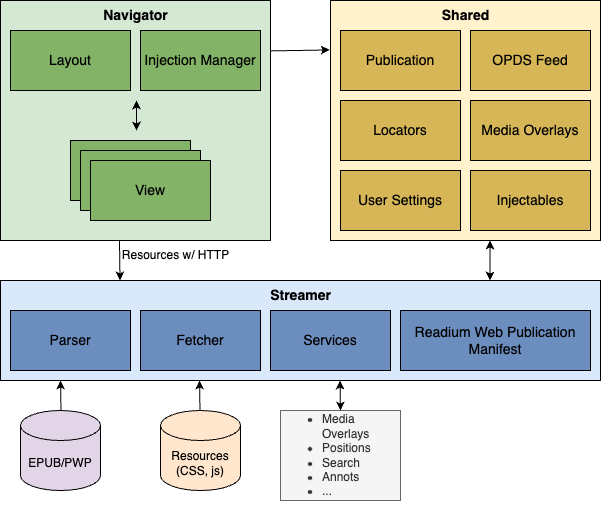
\includegraphics[width=0.7\textwidth]{img/tesi-22-readiumarch.drawio.png}
\caption{Architettura libreria Readium}
\end{figure}

\subsection{Shared}
Come anticipato nel capitolo \ref{ch:ch3} la parte condivisa della applicazione racchiude tutta o una sottoparte della business logic, compresi quindi aspetti "infrastrutturali" specifici della piattaforma target come ad esempio logging, persistenza dei dati e networking. E' infatti in questo modulo che si trova l'implementazione della logica applicativa seguendo le specifiche definite in fase di progettazione (figura \ref{fig:5.4}).\\
Lo schema del database locale è definito utilizzando appositi file, in formato \textit{.sq}, uno per ognuna delle entità che necessita di persistenza: \textit{Highlight}, \textit{Favorite}, \textit{Progression} e \textit{Bookmark}. Tramite il task \textit{generateSqlDelightInterface} fornito dal plugin gradle SqlDelight è possibile generare le relative implementazioni dell'interfaccia \textit{MaggioliEbookDB}, anch'essa autogenerata dal plugin. 

\begin{figure}[H]
\centering
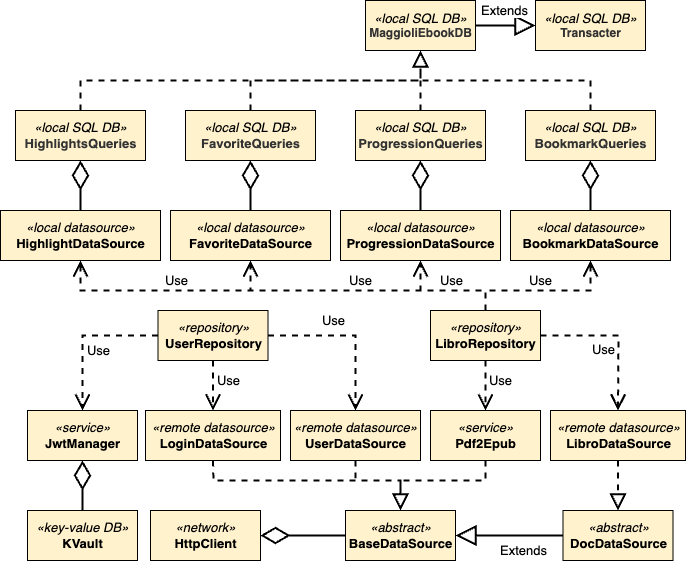
\includegraphics[width=0.9\textwidth]{img/tesi-26-shareduml.drawio.png}
\caption{UML - Diagramma delle classi: Implementazioni data source (persistenza dati e networking)}
\end{figure}

\begin{listing}[H]
\inputminted{sql}{code/5-sqldelight}
\caption{Esempio di definizione schema \textit{Bookmark} tramite sintassi SqlDelight}
\end{listing}

\begin{listing}[H]
\inputminted{kotlin}{code/5-sqldelight1}
\caption{Implementazione autogenerata tramite il plugin gradle SqlDelight della precedente definizione dello schema per l'entità \textit{Bookmark}}
\end{listing}

Tipicamente le librerie per applicazioni sviluppate con Kotlin Multiplatform possono essere utilizzate direttamente dal codice condiviso, come ad esempio KVault, lasciando al compilatore Kotlin il compito di scegliere la giusta implementazione per la piattaforma target durante la fase di compilazione.In altri casi è necessario invece utilizzare il meccanismo \textit{expect/actual} (discusso nel capitolo \ref{ch:ch3}) per definire il comportamento atteso e fornire una implementazione specifica per la piattaforma target.\\
Tale meccanismo è stato utilizzato nello sviluppo della applicazione per poter effettuare dependency injection tramite la libreria Koin dei componenti riguardanti la persistenza dei dati (Kvault e SqlDelight) e l'esecuzione asincrona (CoroutineDispatcher).

\begin{figure}[H]
\centering
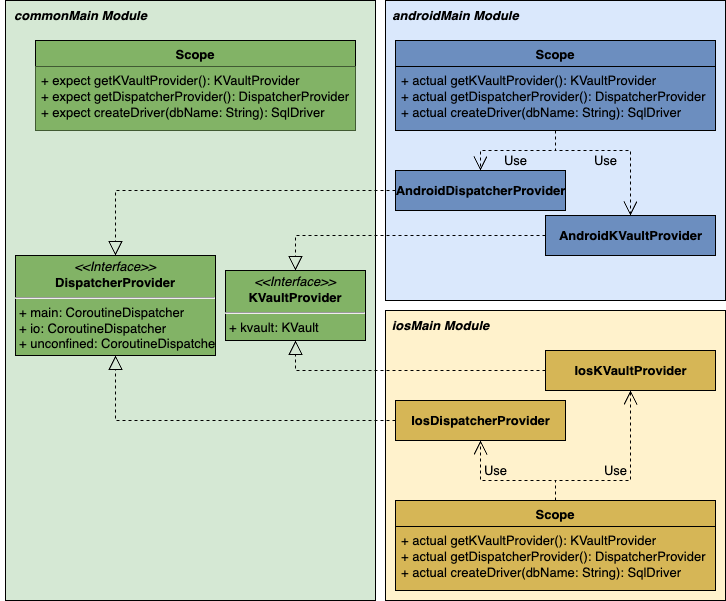
\includegraphics[width=0.9\textwidth]{img/tesi-21-expectactual.drawio.png}
\caption{Strategia \textit{Expect/Actual} adottata per l'implementazione dei servizi infrastrutturali specifici delle piattaforme, persistenza e concorrenza, sfruttando la tecnica \textit{dependency injection}}
\end{figure}

Ogni dipendenza che deve essere iniettata viene inserita all'interno di uno o più moduli, i quali vengono utilizzati da Koin per inizializzare tutto il contesto applicativo. Le dipendenze possono essere principalmente di due tipi:
\begin{itemize}
    \item \textit{Factory} - Ogni volta che la dipendenza viene iniettata ne viene creata una nuova istanza (paragonabile al design pattern Factory Method\footnote{\url{https://en.wikipedia.org/wiki/Factory_method_pattern}}).
    \item \textit{Single} - In tutto il contesto applicativo esiste una sola istanza della dipendenza iniettata (paragonabile al design pattern Singleton\footnote{\url{https://en.wikipedia.org/wiki/Singleton_pattern}}).
\end{itemize}

\begin{listing}[H]
\inputminted{kotlin}{code/5-koin}
\caption{Configurazione Dependency Injection: definizione dei moduli Koin e inizializzazione del contesto applicativo}
\end{listing}

\subsection{androidMaggioliEbookApp}
L'applicazione sviluppata per la piattaforma Android implementa sia lo strato della visualizzazione dei dati utilizzando la business logic fornita dal modulo \textit{Shared} che la logica del \textit{Reader}, visualizzatore dei contenuti digitali tramite il toolkit Kotlin della libreria \textit{Readium}.
\subsubsection{Single-Activity Architecture}
L'architettura scelta per l'implementazione della applicazione Android è basata su sole due activity:
\begin{itemize}
    \item \textit{MainActivity} - Unica activity principale della applicazione.
    \item \textit{ReaderActivity} - Activity secondaria, utilizzata sia per l'interazione che la gestione del lettore di contenuti digitali.
\end{itemize}
Questa tipologia di architettura permette di avere una singola activity che svolge la funzione di "big container" per tutti i fragment che rappresentano le varie schermate della applicazione.

\begin{figure}[H]
\centering
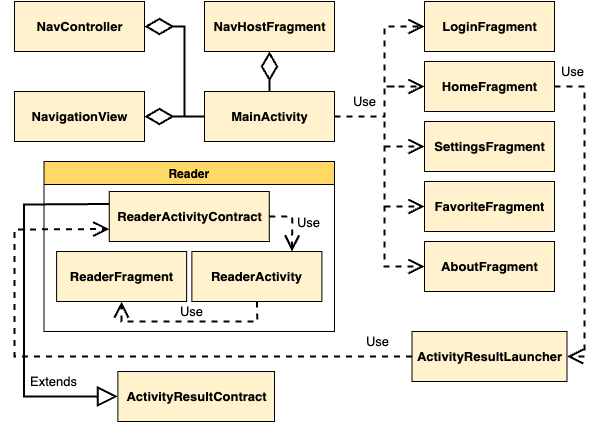
\includegraphics[width=0.7\textwidth]{img/tesi-27-singleactivity.drawio.png}
\caption{UML - Diagramma delle classi: architettura Single-Activity}
\label{fig:5.10}
\end{figure}

La navigazione all'interno della applicazione è gestita tramite la combinazione dei seguenti componenti:
\begin{itemize}
    \item \textit{NavController} - Componente necessario per la gestione delle transizioni da un un fragment all'altro. Quando inizializzato richiede la presenza di un grafo di navigazione tra le risorse XML: tale grafo contiene tutti i fragment che possono essere visualizzati e le possibili transizioni tra di essi.
    \item \textit{NavHostFragment} - Rappresenta il contenitore del fragment in cui ci si trova. Ogni transizione nel grafo corrisponde alla sostituzione del fragment visualizzato con quello di destinazione (sempre che la transizione sia ammessa dal grafo).
    \item \textit{NavigationView} - Permette la visualizzazione del menu dove si trovano i possibili fragment raggiungibili da quello in cui l'utente si trova attualmente. Nel caso della applicazione sviluppata in questo componente si trova il menu laterale con tutte le schermate indicate in fase di progettazione (\textit{Home}, \textit{Settings}, \textit{About} e \textit{Preferiti}).
\end{itemize}

\begin{figure}[H]
\centering
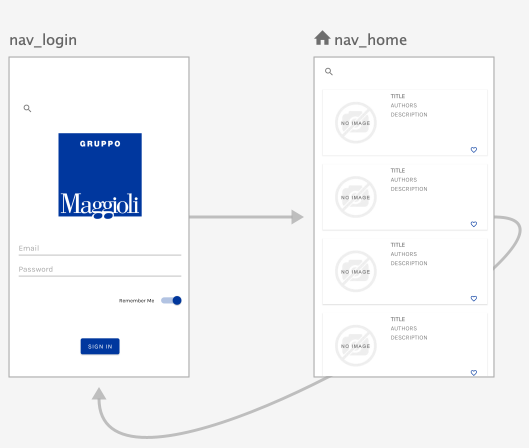
\includegraphics[width=0.7\textwidth]{img/Screenshot 2022-09-07 at 17.12.56.png}
\caption{Screenshot di una sottoparte del navigation graph (renderizzato automaticamente tramite l'IDE Android Studio)}
\label{fig:5.11}
\end{figure}

Come indicato nella figura \ref{fig:5.11} la schermata principale (\textit{Home}) rappresenta la destinazione iniziale del grafo, ovvero la prima schermata che viene visualizzata dalla applicazione. L'autenticazione dell'utente è gestita tramite la navigazione condizionale\footnote{\url{https://developer.android.com/guide/navigation/navigation-conditional}}. Prima di creare la vista del fragment viene effettuato un controllo sulla autenticazione dell'utente: se l'utente non è autenticato viene effettuata una transizione al fragment \textit{Login} per permettere all'utente di autenticarsi e procedere all'utilizzo della applicazione. E' fondamentale in questo scenario ripulire lo stack di navigazione per evitare che l'utente possa tornare indietro alla schermata precedente, ovvero la schermata principale, senza effettuare l'autenticazione.\\

\subsubsection{Paging}
Un altro aspetto importante della architettura è il meccanismo utilizzato sia dalla schermata principale che da quella dei preferiti per mostrare i dati all'utente. Il backend utilizzato fornisce i dati tramite paginazione: in questo modo è possibile indicare in una richiesta la dimensione delle pagine, ovvero quanti elementi devono essere restituiti al massimo in una pagina, e la pagina desiderata. Per poter caricare tali dati dinamicamente in una \textit{RecyclerView}\footnote{\url{https://developer.android.com/reference/kotlin/androidx/recyclerview/widget/RecyclerView}} in modo che l'utente possa effettuare lo scroll illimitato nella schermata si utilizza la libreria \textit{Paging}\footnote{\url{https://developer.android.com/topic/libraries/architecture/paging/v3-overview}} fornita da Android.

\begin{figure}[H]
\centering
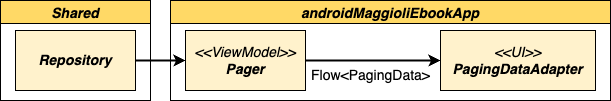
\includegraphics[width=0.75\textwidth]{img/tesi-2-Page-11.drawio.png}
\caption{Flusso generico dei dati dalla sorgente alla UI tramite l'utilizzo della libreria Paging}
\label{paging}
\end{figure}

% aggiungere materiale su paging ecc

I componenti fondamentali della libreria \textit{Paging} sono:
\begin{itemize}
    \item \textit{Pager} - Punto di ingresso principale della libreria con il compito di ottenere nuovi dati quando necessario, ovvero quando l'utente ha scrollato nella schermata fino ad uno specifico punto. Richiede la configurazione di alcuni parametri come la dimensione della pagina, la pagina iniziale e la direzione della paginazione. 
    \item \textit{PagingSource} - Sorgente dei dati paginati. Componente interrogato dal \textit{Pager} ogni volta che sono necessari nuovi dati.
    \item \textit{PagingDataAdapter} - Componente fondamentale per la rappresentazione di dati paginati in una \textit{RecyclerView}.
\end{itemize}

\begin{figure}[H]
\centering
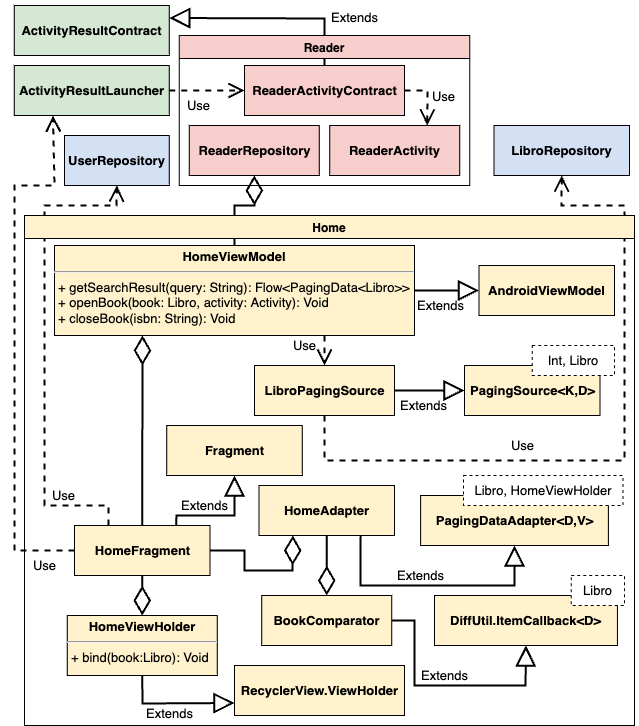
\includegraphics[width=0.7\textwidth]{img/tesi-24-androidviewuml.drawio.png}
\caption{UML - Diagramma delle classi: Paginazione dati nella schermata principale}
\label{paging2}
\end{figure}

\subsection{Reader}
% discutere l'architettura e l'implementazione del reader e mettere qualche screenshot
\begin{figure}[H]
\centering
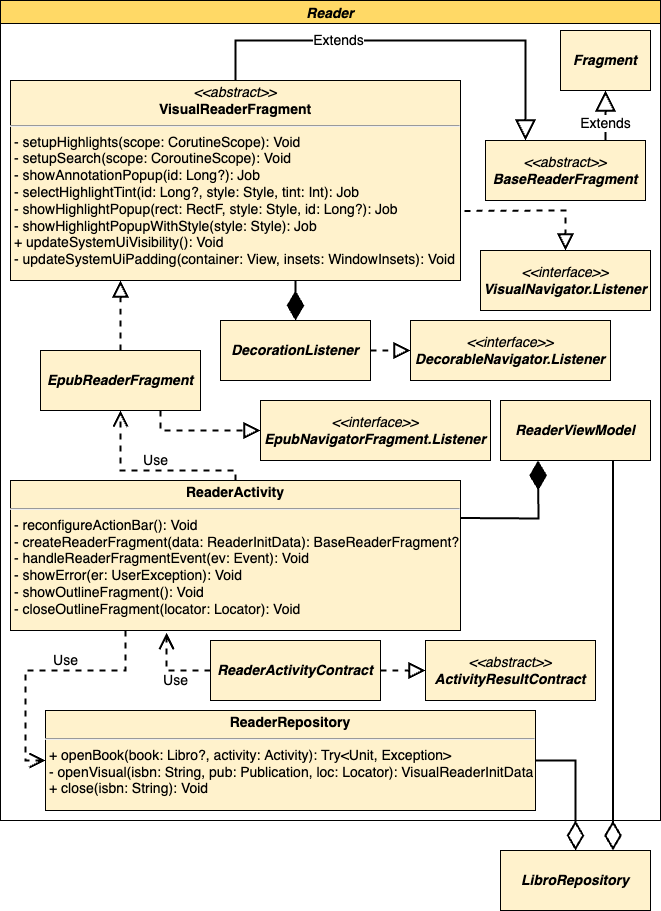
\includegraphics[width=0.8\textwidth]{img/tesi-2-Page-16.drawio.png}
\caption{UML - Diagramma delle classi: Reader}
\label{reader}
\end{figure}

\subsection{iosMaggioliEbookApp}